\documentclass[17pt, t, aspectratio=169, xcolor=table]{beamer}

% To have print without pause
% \documentclass[handout, 17pt, t, aspectratio=169, xcolor=table]{beamer}

\usepackage[utf8]{inputenc}
\usepackage{hyperref}

% Change the presentation layout
\usetheme{Madrid}

% Change the caption size of figure
\usepackage[font=small,skip=4pt]{caption}
\usepackage[symbol]{footmisc}

% Font
\usepackage{plex-sans}

\usepackage[style=numeric,backend=biber,
            doi=false,isbn=false,url=false,eprint=false]{biblatex}
\usepackage{latexsym,xcolor,multicol,booktabs,calligra}
\usepackage{amssymb,amsfonts,amsmath,amsthm,mathrsfs,mathptmx}
\usepackage{graphicx,pstricks,listings,stackengine}
% \usefonttheme[onlymath]{serif}

\usepackage[caption=false]{subfig}
\usepackage{tabularx}
\usepackage{booktabs}

\usepackage{color, colortbl}

% Define color for highlighted table
\definecolor{TableHighLight}{RGB}{190, 250, 196}

\setbeamertemplate{navigation symbols}{}
% \setbeamertemplate{footline}[frame number]
\setbeamertemplate{bibliography item}{\insertbiblabel}
% \setbeamertemplate{footnote}{\insertfootnotetext}

\let\oldfootnotesize\footnotesize
\renewcommand*{\footnotesize}{\oldfootnotesize\tiny}

\DeclareCiteCommand{\footpartcite}[\mkbibfootnote]
{\usebibmacro{prenote}}%
{\usebibmacro{citeindex}%
    \mkbibbrackets{\usebibmacro{cite}}%
    \setunit{\addnbspace}
    \printnames{labelname}%
    \setunit{\labelnamepunct}
    \printfield[citetitle]{title}%
    \newunit
    \printfield[]{year}}
{\addsemicolon\space}
{\usebibmacro{postnote}}

\setbeamertemplate{footnote}{\insertfootnotetext}
\setbeamertemplate{caption}[numbered]

% \usepackage[style=numeric, sorting=none]{biblatex}
 % Insert the structure.tex file which contains the majority of the structure behind the template

%------------------------------------------------------------
%This block of code defines the color theme
\definecolor{ThemeColor}{RGB}{ 40,135, 50} % Elektro- und Informationstechnik
% \definecolor{ThemeColor}{RGB}{ 25,130,130} % Architektur- und Bauwesen
%\definecolor{ThemeColor}{RGB}{ 40,105,175} % Maschinenbau und Mechatronik
%\definecolor{ThemeColor}{RGB}{ 30, 70,150} % Wirtschaftswissenschaften
%\definecolor{ThemeColor}{RGB}{100, 55,140} % Informatik und Wirtschaftsinformatik
%\definecolor{ThemeColor}{RGB}{140, 45,130} %Informationsmanagement und Medien
\usecolortheme[named=ThemeColor]{structure}

%------------------------------------------------------------
%%%% Definition of Layout metrics

\newcommand{\covertextsize}{44}
\newcommand{\titletextsize}{32}
\newcommand{\contenttextsize}{18}

\newcommand{\leftmarginpos}{0.9335cm}

\newcommand{\topmargintitle}{-0.825cm}

\newcommand{\topmargincontent}{3.5cm}

\newcommand{\maximumwidth}{31.912cm}
\newcommand{\maximumheight}{12.613cm}

\newcommand{\columnmaxwidth}{15.45cm}
\newcommand{\secondcolumnstart}{17.395cm}

\newcommand{\captionsize}{normalsize}
\usepackage[font=\captionsize,skip=4pt]{caption}

\definecolor{TableHighLight}{RGB}{190, 250, 196}

%%%%

\newcommand{\germanlipsum}{
    Lorem ipsum ist ein pseudo-Lateinischer Text für Webdesign, 
    Typografie, Layout und Printmedien. Er ersetzt Deutsch um Designelemente 
    gegenüber dem Inhalt hervorzuheben, hat also die Funktion als Platzhalters 
    in Layouts um dem Betrachter eine vorläufige Vorstellung der endgültigen Fassung 
    zu vermitteln. Buchstaben, Worte, Wort- und Satzlängen bilden ungefähr das Schriftbild eines 
    lateinischen Texts wieder. Latein war in früheren Jahrhunderten eine häufig 
    genutzte Sprache verschiedener Textgattungen, z. B. wissenschaftlicher Werke, 
    Ratgeber, oder auch der sogenannten Erbauungsliteratur. Um die Aufmerksamkeit des 
    Lesers ausschließlich auf das Schriftbild zu lenken wird auch ein zufälliger Sinn 
    durch Wort- oder Satzkombinationen vermieden.
}
\newcommand{\germanlipsumshort}{
    Lorem ipsum ist ein pseudo-Lateinischer Text für Webdesign, 
    Typografie, Layout und Printmedien.
}

\addbibresource{bibliography.bib}

%End of title page configuration block
%------------------------------------------------------------

\makeatletter
\def\@makefnmark{}

\begin{document}

\EITCoverVI{Wilkommen}{Vorname Nachname}

\EITTableOfContent{Inhaltsverzeichnis}{2}

%%%%%%%%%%%%%%%%%%%%%%%%%%%
%%%%%%%% Skip this part
\section{EIT Präsentation Layout}


\EITHeadline{EIT Präsentation Layout}{
	\begin{tikzpicture}
		\draw (0,0) rectangle (1in, 1in);
	\end{tikzpicture}

}
%%%%%%%% Skip this part
%%%%%%%%%%%%%%%%%%%%%%%%%%%

\section{EIT Präsentation}

\EITHeadlineFT{EIT Präsentation}{
	\germanlipsum
}




\EITHeadlineFT{EIT Präsentation mit Liste}{
	\begin{itemize}
		\item \germanlipsumshort
		\item \germanlipsumshort
		\item \germanlipsumshort
		\item \germanlipsumshort
	\end{itemize}
}

\EITHeadlineFT{EIT Präsentation mit Liste}{
	\begin{itemize} [<+->]
		\item \germanlipsumshort
		\item \germanlipsumshort
		\item \germanlipsumshort
		\item \germanlipsumshort
	\end{itemize}
}

\EITHeadlineFT{EIT Präsentation mit Liste}{
	\begin{itemize} [<+- | alert@+>]
		\item \germanlipsumshort
		\item \germanlipsumshort
		\item \germanlipsumshort
		\item \germanlipsumshort
	\end{itemize}
}


\section{EIT Präsentation mit Equation}
\EITHeadlineFT{EIT Präsentation mit Equation}
{
	Reference to Eq. \ref{eq:first_eq}.

	\begin{equation}
		f(x)=\left\{\begin{aligned}  & \mathrm{e}^{|x|} &  & \text{si $|x-x^0|\leq 1/2$} \\
                 & 0                &  & \text{si $|x-x^0|> 1/2$}\end{aligned}\right.
		\label{eq:first_eq}
	\end{equation}
}

\section{EIT Präsentation mit 2 Spalten}
\EITHeadlineFT{EIT Präsentation mit 2 Spalten}
{
	\placetextbox{\leftmarginpos}{-\topmargincontent}{\columnmaxwidth}{
		\germanlipsum
	}
	\placetextbox{\secondcolumnstart}{-\topmargincontent}{\columnmaxwidth}{
		\germanlipsum
	}
}

\EITHeadlineFT{EIT Präsentation mit ``Floating'' Text}
{
	\placetextbox{\leftmarginpos + 3cm}{-\topmargincontent - 1cm}{\columnmaxwidth}{
		\germanlipsum
	}
}

\section{EIT Präsentation mit Tabelle}
\EITHeadlineFT{EIT Präsentation mit Tabelle}{
	\begin{table}
		\begin{center}
			\begin{tabular}{||c | c c | c c c||}
				\hline
				\# & A & B & C \textsuperscript{\dag} & D \textsuperscript{\S} & E\textsuperscript{\dag\dag} \\ [0.5ex]
				\hline\hline
				1  & A & B & C                        & D                      & E                           \\
				\hline
				2  & A & B & C                        & D                      & E                           \\
				\hline
				\rowcolor{TableHighLight}
				5  & A & B & C                        & D                      & E                           \\
				\hline

				\rowcolor{TableHighLight}
				6  & A & B & C                        & D                      & E                           \\ [0.2ex]
				\hline
			\end{tabular}
			\caption{\label{table:highlight} die Tabelle }
		\end{center}
	\end{table}
}

\EITHeadlineFT{EIT Präsentation mit ``Floating'' Tabelle}{
	\placetextbox{0.2\paperwidth}{0}{\maximumwidth}{
		\begin{table}
			\begin{tabular}{||c | c c | c c c||}
				\hline
				\# & A & B & C \textsuperscript{\dag} & D \textsuperscript{\S} & E\textsuperscript{\dag\dag} \\ [0.5ex]
				\hline\hline
				1  & A & B & C                        & D                      & E                           \\
				\hline
				2  & A & B & C                        & D                      & E                           \\
				\hline
				\rowcolor{TableHighLight}
				5  & A & B & C                        & D                      & E                           \\
				\hline

				\rowcolor{TableHighLight}
				6  & A & B & C                        & D                      & E                           \\ [0.2ex]
				\hline
			\end{tabular}
			\caption{\label{table:highlight1} die Tabelle }
		\end{table}
	}
}

\section{EIT Präsentation mit Bild}
\EITHeadlineFT{EIT Präsentation mit Bild}
{
	\placetextbox{\leftmarginpos}{-\topmargincontent}{\maximumwidth}{
		\picdims[width=\maximumwidth]{\maximumwidth}{\maximumheight}{Pictures/csm_HKA_FK-EIT_2017-9363_a9e6e1d039.jpg}
	}
}


\EITHeadlineFT{EIT Präsentation 2 Bilder}{
	\placetextbox{\leftmarginpos}{-\topmargincontent}{\columnmaxwidth}{
		\picdims[width=\paperwidth]{\columnmaxwidth}{\maximumheight}{Pictures/csm_HKA_FK-EIT_2017-9363_a9e6e1d039.jpg}
	}

	\placetextbox{\secondcolumnstart}{-\topmargincontent}{\columnmaxwidth}{
		\picdims[width=\paperwidth]{\columnmaxwidth}{\maximumheight}{Pictures/csm_HKA_FK-EIT_2017-9363_a9e6e1d039.jpg}
	}
}

\EITHeadlineFT{EIT Präsentation mit ``Floating'' Bilder}
{
	\placetextbox{\leftmarginpos + 0.2\paperwidth}{-\topmargincontent - 5cm}{\maximumwidth}{
		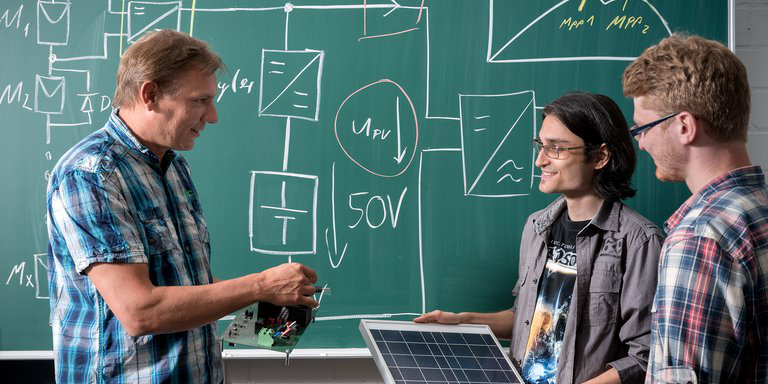
\includegraphics[scale=0.5]{Pictures/csm_HKA_FK-EIT_2017-9363_a9e6e1d039.jpg}
	}
}



\EITHeadlineFT{EIT Präsentation mit Text und Bilder}{

	\placetextbox{\leftmarginpos}{-\topmargincontent}{\columnmaxwidth}{
		\lipsum[2]
	}

	\placetextbox{\secondcolumnstart}{-\topmargincontent}{\columnmaxwidth}{
		\picdims[width=\paperwidth]{\columnmaxwidth}{\maximumheight}{Pictures/csm_HKA_FK-EIT_2017-9363_a9e6e1d039.jpg}
	}
}

\EITHeadlineFT{}{

	\placetextbox{0cm}{0cm}{\paperwidth}{
		\picdims[width=\paperwidth]{\paperwidth}{16cm}{Pictures/csm_HKA_FK-EIT_2017-9363_a9e6e1d039.jpg}
	}

}

\EITHeadlineFT{References}{
	\begin{itemize}
		\item \fullcite{article_key}
		\item \fullcite{book_key}
	\end{itemize}
}

\end{document}